\documentclass[titlepage, 12pt]{article}

\usepackage[margin=1.25in]{geometry}
\usepackage{fancyhdr}
\pagestyle{fancy}

\usepackage{graphicx}

\usepackage{float}
\restylefloat{table}
\usepackage[
    bookmarksopen,
    bookmarksdepth=2,
    breaklinks=true
    ]{hyperref}

\newcommand{\authorName}{Nicola Pfister \& Jonas Meise}


\lhead{WaaS - WebE FFHS}
\rhead{\authorName}

\author{\authorName}
\title{WaaS - Documentation \\ \medskip \large WebE - FFHS}

\begin{document}

\maketitle

\pagebreak

\renewcommand{\contentsname}{Table of Contents}

\tableofcontents

\pagebreak

\section{Introduction}

This is the documentation of the project WaaS, which was done as part of the module Web Engineering at the FFHS. The goal of the project is to create a concept and implement a web application which fullfills at least the following criteria:

\begin{itemize}
    \item Basic user authentication (register, login/logout, delete and update user)
    \item Public and dynamic/user specific content
    \item Persist user data (in database or file)
    \item Basic validation and error handling
    \item Support for sessions and cookies
\end{itemize}

\section{Requirements Engineering\label{sectionRequirementsEngineering}}

This chapter contains purpose and context of the Webapplication WaaS aswell as the functional and non-functional requirements.

\begin{itemize}
  \item \textbf{Name of the application:} WaaS
  \item \textbf{Purpose:} WaaS is a webapplication that allows it's users to crawl urls with specified search patterns and notifies them as it finds the pattern.
  \item \textbf{Names:} Nicola Pfister, Jonas Meise
\end{itemize}

\subsection{Purpose \& Context}

WaaS (Webcrawler as a Service) is a service, that allows users to keep track of news on their favourite websites, by giving them the possibility to create "crawls". A crawl is defined with a URL, a search pattern and an email address. WaaS will regularly check those URLs for the given search patterns and notifies the users via their email address when it finds the pattern it was searching for.
\medskip \\
The following graphic visualizes the context of the app with it's use cases.
\begin{figure}[H]
  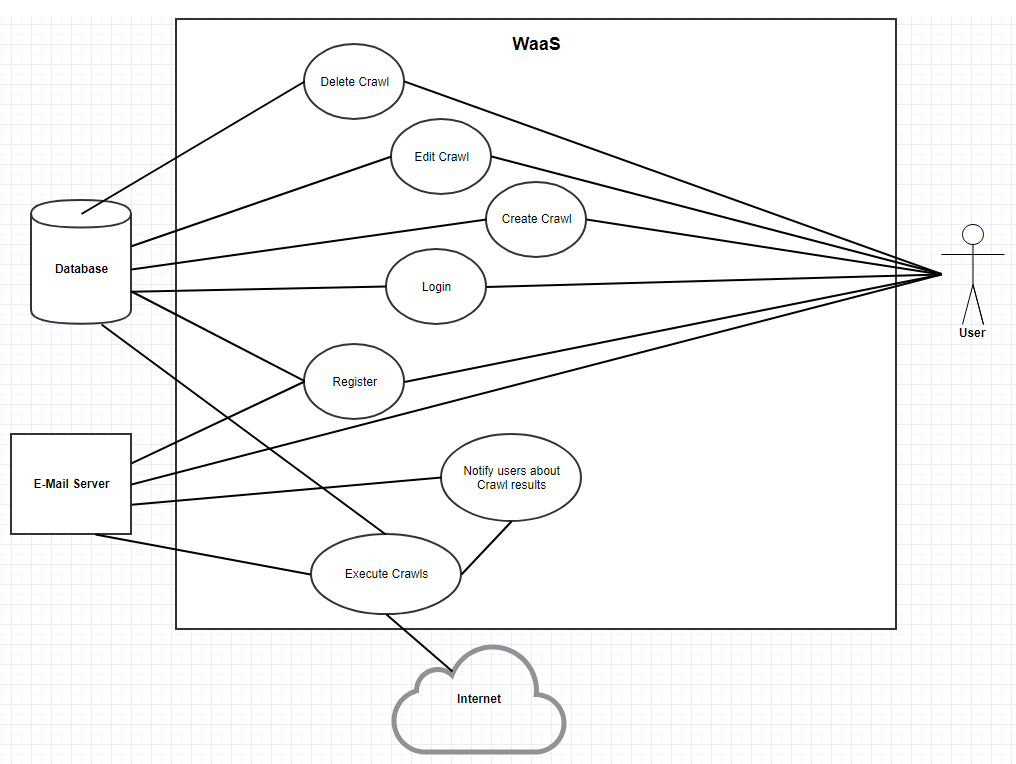
\includegraphics[width=\linewidth]{UseCaseDiagram.PNG}
  \caption{Use Case Diagram}
  \label{fig:useCaseDiagram}
\end{figure}

\subsection{Functional Requirements}

The following chapter contains the functional requirements for WaaS.

\subsubsection{Target Group}

The target group of WaaS are mainly people that are regularly checking websites for news. That concludes people of all ages who understand what a webcrawler is. It can also be used from people who want to check wether or not the new episode of their favourite tv series is already online. All of those people are generally expected to have some basic skills in the field of IT or are at least interested in it.

\subsubsection{{Use Cases}}

\begin{table}[H]
  \begin{center}

    \begin{tabular}{p{4cm}|p{10cm}}
      \textbf{UST-1 Register}                                                                                                        \\
      \hline
      Goal             & A user registers a useraccount for WaaS.                                                                    \\
      \hline
      Actors           & Eventual user of WaaS                                                                                       \\
      \hline
      Precondition     & The user owns a valid email address that is not yet used for an existing useraccount                        \\
      \hline
      Trigger          & Click on the button: "Register"                                                                             \\
      \hline
      Main path        &
      \begin{itemize}
        \item [1] The user clicks the button: "SignUp".
        \item [2] The user enters his credentials into the register form (email address, and password).
        \item [3] The user clicks on: "Register".
        \item [4] WaaS creates a useraccount entry in the database.
        \item [5] The user gets redirected to the Login Page.
      \end{itemize}                                                                                                      \\
      \hline
      Alternative path &
      \begin{itemize}
        \item [1a] The user enters a invalid input data.
        \item [2a] A validation error message shows up.
      \end{itemize}                                                                                                      \\
      \hline
      Postcondition    & A new useraccount was created in the database with the credentials the user entered into the register form. \\
    \end{tabular}

    \caption{UST-1}
    \label{table:UST-1}

  \end{center}
\end{table}

\begin{table}[H]
  \begin{center}

    \begin{tabular}{p{4cm}|p{10cm}}
      \textbf{UST-2 Login}                                                              \\
      \hline
      Goal             & A user logs in with an existing user account.                  \\
      \hline
      Actors           & registered users                                               \\
      \hline
      Precondition     & UST-\ref{table:UST-1}                                          \\
      \hline
      Trigger          & Click on the button: "LogIn"                                   \\
      \hline
      Main path        &
      \begin{itemize}
        \item [1] The user enters a valid email address an password into the login form.
        \item [2] The user clicks on the button: "LogIn".
      \end{itemize}                                                         \\
      \hline
      Alternative path &
      \begin{itemize}
        \item [1a] The user enters a invalid input data.
        \item [2a] A validation error message shows up.
      \end{itemize}                                                         \\
      \hline
      Postcondition    & The user is now logged in and is situated on the overview page \\
    \end{tabular}

    \caption{UST-2}
    \label{table:UST-2}

  \end{center}
\end{table}

\begin{table}[H]
    \begin{center}
  
      \begin{tabular}{p{4cm}|p{10cm}}
        \textbf{UST-3}\\ \textbf{Create Crawl}                                            \\
        \hline
        Goal             & A user creates a new crawl.                  \\
        \hline
        Actors           & logged in users                                               \\
        \hline
        Precondition     & UST-\ref{table:UST-1} \& UST-\ref{table:UST-2}                \\
        \hline
        Trigger          & Click on the button: "+"                                   \\
        \hline
        Main path        &
        \begin{itemize}
          \item [1] The user enters a URL and a search pattern into the New Crawl form.
          \item [2] The user clicks on the button: "Save".
        \end{itemize}                                                         \\
        \hline
        Alternative path &
        \begin{itemize}
          \item [1a] The user clicks the button "Cancel".
          \item [2a] The user redirected back to the overview page.
        \end{itemize}                                                         \\
        \hline
        Postcondition    & The newly created crawl is persisted in the database \& The new crawl gets displayed on the users overview page. \\
      \end{tabular}
  
      \caption{UST-3}
      \label{table:UST-3}
  
    \end{center}
  \end{table}

  \begin{table}[H]
    \begin{center}
  
      \begin{tabular}{p{4cm}|p{10cm}}
        \textbf{UST-4}\\ \textbf{Delete Crawl}                                            \\
        \hline
        Goal             & A user deletes an existing crawl.                  \\
        \hline
        Actors           & logged in user                                               \\
        \hline
        Precondition     & UST-\ref{table:UST-3}                                     \\
        \hline
        Trigger          & Click on the delete crawl button.                            \\
        \hline
        Main path        &
        \begin{itemize}
          \item [1] The user clicks on the delete button of the crawl he wishes to remove.
          \item [2] A confirmation dialogue is shown.
          \item [3] The user clicks the "Delete" button.
          \item [4] The crawl gets deleted from the database.
        \end{itemize}                                                         \\
        \hline
        Alternative path &
        \begin{itemize}
          \item [3a] The user clicks the button "Cancel".
          \item [4a] The confirmation dialogue closes.
        \end{itemize}                                                         \\
        \hline
        Postcondition    & The crawl is deleted from the database \& The crawl does not get displayed on the users overview page anymore. \\
      \end{tabular}
  
      \caption{UST-4}
      \label{table:UST-4}
  
    \end{center}
  \end{table}

  \begin{table}[H]
    \begin{center}
  
      \begin{tabular}{p{4cm}|p{10cm}}
        \textbf{UST-5}\\ \textbf{Edit Crawl}                                            \\
        \hline
        Goal             & A user edits an existing crawl.                  \\
        \hline
        Actors           & logged in user                                               \\
        \hline
        Precondition     & UST-\ref{table:UST-3}                                     \\
        \hline
        Trigger          & Click on the edit crawl button.                            \\
        \hline
        Main path        &
        \begin{itemize}
          \item [1] The user clicks on the edit button of the crawl he wishes to edit.
          \item [2] The Edit Crawl form is shown.
          \item [3] The user changes the Crawls URL.
          \item [4] The user clicks "Save".
          \item [5] The changes get persisted in the database.
        \end{itemize}                                                         \\
        \hline
        Alternative path &
        \begin{itemize}
          \item [4a] The user clicks the button "Cancel".
          \item [5a] The Edit Crawl form closes.
        \end{itemize}                                                         \\
        \hline
        Postcondition    & The updated crawl gets displayed on the users overview page. \\
      \end{tabular}
  
      \caption{UST-5}
      \label{table:UST-5}
  
    \end{center}
  \end{table}

\subsection{Non-functional Requirements}

\begin{enumerate}
  \item \textbf{Performance}
        \begin{enumerate}
          \item For user interactions, the application should respond 99\% of the requests in 2 seconds.
          \item The application should score at least 40 points of performance in Google Chromes inbuilt Lighthouse audit.
        \end{enumerate}
  \item \textbf{Usability}
        \begin{enumerate}
          \item If the application experiences any kind of error or delay, users should be made aware of this.
          \item When a website that is subject to a Crawl changes to contain the looked for pattern, users should receive a notification within an hour.
        \end{enumerate}
  \item \textbf{Other non-functional requirements}
        \begin{enumerate}
          \item The application should be implemented according to best practices and should therefore score 100 points in the best practices section of the Lighthouse audit.
          \item Due to the use of relational database technology, horizontal scalability is too big of a task to be realized in the given time frame and is therefore outside of the scope of this project.
        \end{enumerate}
\end{enumerate}

\pagebreak

\listoftables
\listoffigures

\pagebreak

\bibliography{uni}
\bibliographystyle{ieeetr}




\end{document}
